%%% Template originaly created by Karol Kozioł (mail@karol-koziol.net) and modified for ShareLaTeX use

%%%------------------------------------------------------------------------------------------------%%%
%%%------------------------------------%%%     PREAMBLE     %%%------------------------------------%%%
%%%------------------------------------------------------------------------------------------------%%%

\documentclass[twoside=false,a4paper,11pt]{article}

\usepackage[T1]{fontenc}
\usepackage[utf8]{inputenc}
\usepackage{graphicx}
\usepackage{xcolor}

\usepackage{tgtermes}



\usepackage[
pdftitle={CPSC 471 Final Report}, 
pdfauthor={Timothy Mealey, Ben Roberts, Cory Jensen, Scott Saunders, University of Calgary},
colorlinks=true,linkcolor=blue,urlcolor=blue,citecolor=blue,bookmarks=true,
bookmarksopenlevel=2]{hyperref}
\usepackage{amsmath,amssymb,amsthm,textcomp}

\usepackage{enumitem}

\usepackage{multicol}
\usepackage{tikz}
\usetikzlibrary{shapes,positioning,calc}
\colorlet{lightgray}{gray!20}

\usepackage{geometry}
\geometry{total={210mm,297mm},
left=25mm,right=25mm,%
bindingoffset=0mm, top=20mm,bottom=20mm}

\linespread{1.3}

\newcommand{\linia}{\rule{\linewidth}{0.5pt}}

% custom theorems if needed
\newtheoremstyle{mytheor}
    {1ex}{1ex}{\normalfont}{0pt}{\scshape}{.}{1ex}
    {{\thmname{#1 }}{\thmnumber{#2}}{\thmnote{ (#3)}}}

\theoremstyle{mytheor}
\newtheorem{defi}{Definition}

% my own titles
\makeatletter
\renewcommand{\maketitle}{
\begin{center}
\vspace{2ex}
{\huge \textsc{\@title}}
\vspace{1ex}
\\
\linia\\
\@author \hfill \@date
\vspace{4ex}
\end{center}
}
\makeatother
%%%

% custom footers and headers
\usepackage{fancyhdr,lastpage}
\pagestyle{fancy}
\lhead{}
\chead{}
\rhead{}
\lfoot{Final Report}
\cfoot{}
\rfoot{Page \thepage\ /\ \pageref*{LastPage}}
\renewcommand{\headrulewidth}{0pt}
\renewcommand{\footrulewidth}{0pt}
%


%%%------------------------------------------------------------------------------------------------%%%
%%%------------------------------------%%%     DOCUMENT     %%%------------------------------------%%%
%%%------------------------------------------------------------------------------------------------%%%

\newcommand{\tuple}[2]{\{ #1 | #2 \}}
\newcommand{\domain}[2]{\{ (#1) | #2 \}}

\newcommand{\quantifier}[2]{(\ensuremath{#1}#2)}
\newcommand{\one}[1]{\quantifier{\exists}{#1}}
\newcommand{\all}[1]{\quantifier{\forall}{#1}}

\begin{document}

\title{CPSC 471 Final Report}
\author{Timothy Mealey, Ben Roberts, Cory Jensen, Scott Saunders}
\date{\today}
\maketitle

\section*{Abstract}

``An abstract of no more than 300 words.''

\section*{Introduction}

``Describe the problem or task your database was designed to address.
Describe (briefly) the system you have created to address the problem or task.''

\section*{Design}

\subsection*{Users}

``Discuss the different users of your system. Your discussion in this section should be considerably more detailed than what you described for the presentation - this section should describe a complete transaction collection and, consequently, provide a complete picture of the functionality offered by your system.''

\begin{enumerate}
	\item Course Browsing
	A user interested in courses offered by the University of Calgary can navigate to the Dauwtrappen website. Once on the website, a series of SQL queries are executed which load the entire course list. These queries are executed in alphabetical order by department so that the user can begin interacting with the system before all of the data is loaded.
	Once some or all of the course data is loaded, the user can either browse through the courses using the course tree or perform a search for preferred courses by department, course numbers, and course names. Courses that fulfill their selection/search criteria display the corresponding course information such as their name and number, description, prerequisites, and when/whether they are offered.

	A user would use the Dauwtrappen website as opposed to the UofC Calender website for 3 reasons, some of which have already been mentioned:
	Firstly, the intuitive search tool.
	Secondly, the UofC Calender only mentions if courses are offered in even/odd years, but does not state which semester the courses will actually be offered in, whereas the Dauwtrappen course list does just that.
	Thirdly, the overall integration of all aspects of the Dauwtrappen website.

	\item Schedule Building
	A student or perspective student can navigate to the schedule building page of the website in order to get organized for the upcoming semester. Again, a series of SQL queries are executing which loads the course data in a cascading fashion. The user can browse through the list or use the same search tool that is present in the course selection. 
	The user can then click on a course to add it to the selected courses panel on the right side of the screen. This panel will then display the various lectures, tutorials, and labs available for that course, as well as their corresponding times. The user can individually click on these sections to add them to their schedule. To remove a selected course, the user can click the little X button on the course. This will remove it from the selected course panel and any selected sections will be removed from the schedule itself. 
	Once the user completes their schedule, they can click the save button to save their schedule to the database. They can give it a name if they wish, but this is not required.
	They may also load schedules from the database by pressing the load button and selecting the schedule they wish to load.  

	Currently the user login system is not session based, so all schedules are accessible by all users of the system.

	\item Login System

	A user who wishes to login to the website navigates to the login page. Once there, if they already have an account, they can enter their username (email) and their password, then press to login button. This executes an SQL query to confirm that have an account and that they entered the correct password. If they do not have an account, they can enter their email and a password and press the create account button. This will create an entry in the database table for that user, and they will now be able to login to the system.

	The website does not currently have sessions, so logging in does not carry over to the courses or schedule page. 

\end{enumerate}

\subsubsection*{Log In}
\subsubsection*{Course Search}
\subsubsection*{Schedule Creator}

\subsection*{Entity Relationship Diagram}

\includegraphics[width=\textwidth]{ERDiagram.png}

``Any changes that were made since the presentation should be clearly indicated.''

\section*{Implementation}

\subsection*{Relational Schema Diagram}

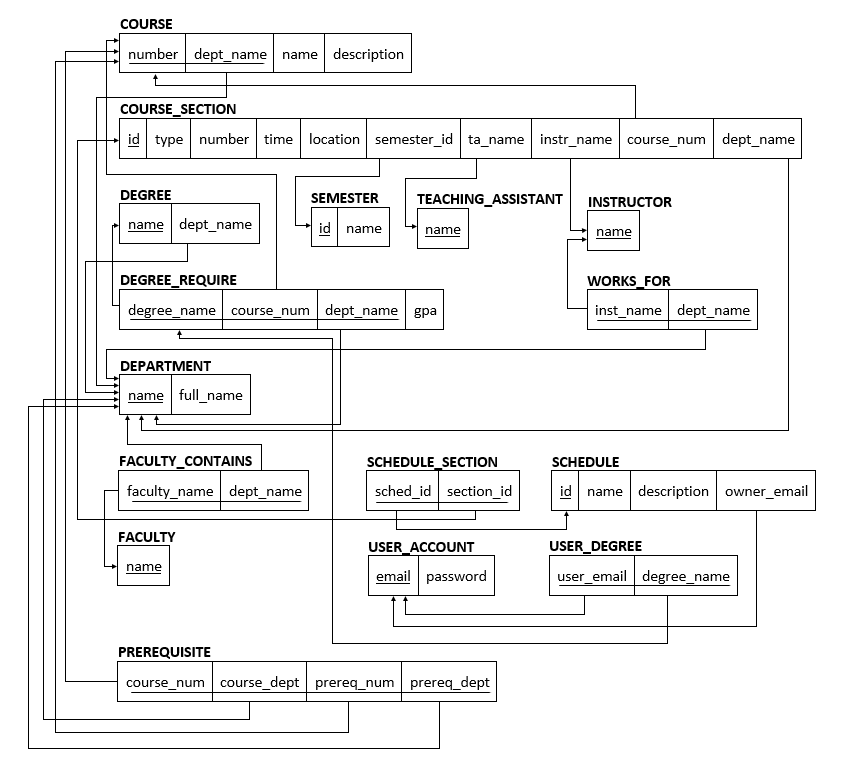
\includegraphics[width=\textwidth]{RelationalSchemaDiagram.png}

``Discuss any significant or unusual decisions made during this process.''

\subsection*{Database Management System}

``Describe the DBMS you selected for the implementation	of the project, and include the SQL statements for each of the transactions implemented. It is not necessary to discuss these transactions in relational algebra or calculus.''

\subsection*{User Interface}

``Present a brief description of your interface design, including several screenshots.''

\end{document}